\thispagestyle{empty}
\subsection{Stack (Array version)}
\subsubsection*{`push' operation}
\begin{figure}[!ht]
	\centering
	\begin{subfigure}{0.41\textwidth}
		\centering
		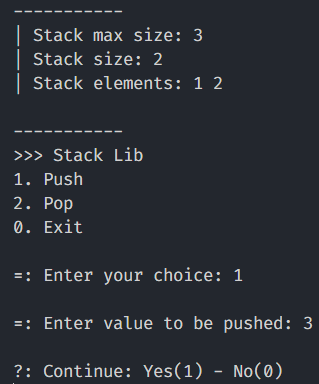
\includegraphics[width=\textwidth]{imgs/StackArray/push/normal.png}
		\caption{Normal test cases}\label{fig:stack_arr_push_normal}
	\end{subfigure}
	\hfill
	\begin{subfigure}{0.54\textwidth}
		\centering
		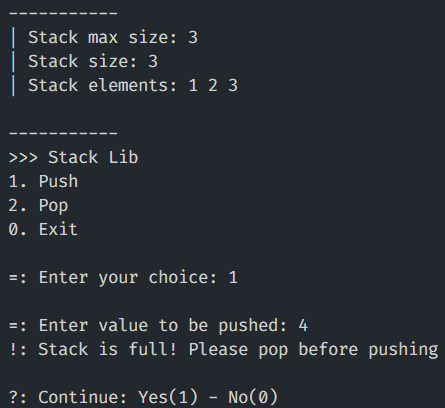
\includegraphics[width=\textwidth]{imgs/StackArray/push/full.png}
		\caption{When the stack is full}\label{fig:stack_arr_push_full}
	\end{subfigure}
	\hfill
	\begin{subfigure}{0.75\textwidth}
		\centering
		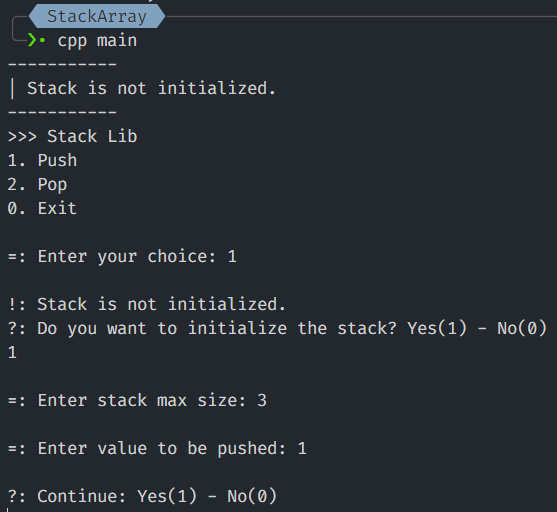
\includegraphics[width=\textwidth]{imgs/StackArray/push/empty.png}
		\caption{When the stack is uninitialized}\label{fig:stack_arr_push_empty}
	\end{subfigure}
	\caption{Screenshots of Stack (Array version) `push' operation.}\label{fig:stack_arr_push_cases}
\end{figure}
\subsubsection*{`pop' operation}
\begin{figure}[!ht]
	\centering
	\begin{subfigure}{0.58\textwidth}
		\centering
		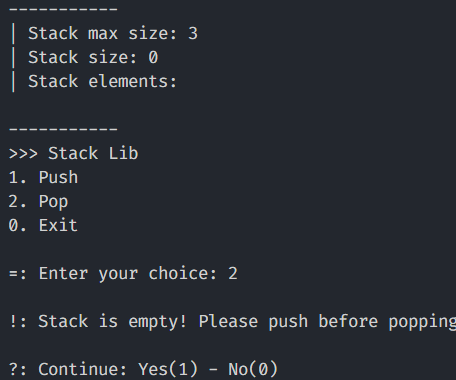
\includegraphics[width=\textwidth]{imgs/StackArray/pop/empty.png}
		\caption{When the stack is empty}\label{fig:stack_arr_pop_empty}
	\end{subfigure}
	\hfill
	\begin{subfigure}{0.39\textwidth}
		\centering
		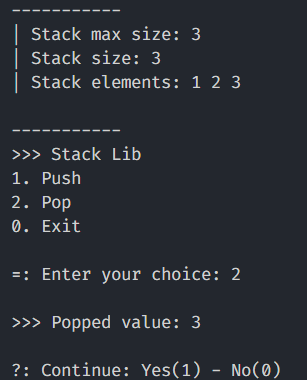
\includegraphics[width=\textwidth]{imgs/StackArray/pop/normal.png}
		\caption{Normal test cases}\label{fig:stack_arr_pop_normal}
	\end{subfigure}
	\caption{Screenshots of Stack (Array version) `pop' operation.}\label{fig:stack_arr_pop_cases}
\end{figure}

\pagebreak
\subsection{Stack (Linked List version)}
\subsubsection*{`push' operation}
\begin{figure}[!ht]
	\centering
	\begin{subfigure}{0.55\textwidth}
		\centering
		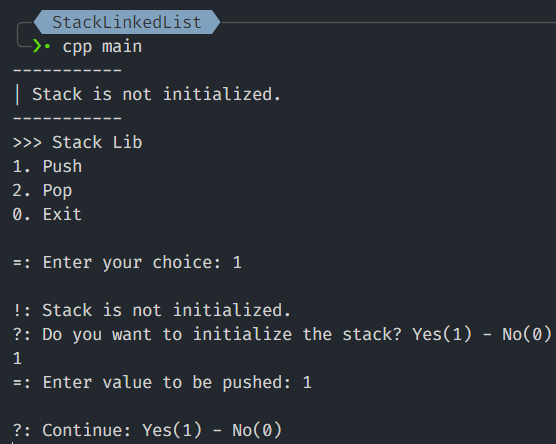
\includegraphics[width=\textwidth]{imgs/StackLinkedList/push/empty.png}
		\caption{When the stack is uninitialized}\label{fig:stack_ll_push_empty}
	\end{subfigure}
	\hfill
	\begin{subfigure}{0.43\textwidth}
		\centering
		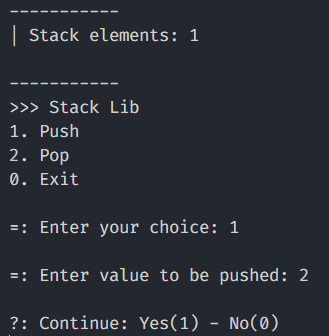
\includegraphics[width=\textwidth]{imgs/StackLinkedList/push/normal.png}
		\caption{Normal test cases}\label{fig:stack_ll_push_normal}
	\end{subfigure}
	\caption{Screenshots of Stack (Linked List version) `push' operation.}\label{fig:stack_ll_push_cases}
\end{figure}
\subsubsection*{`pop' operation}
\begin{figure}[!ht]
	\centering
	\begin{subfigure}{0.59\textwidth}
		\centering
		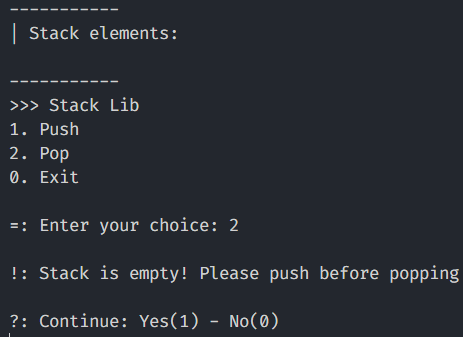
\includegraphics[width=\textwidth]{imgs/StackLinkedList/pop/empty.png}
		\caption{When the stack is empty}\label{fig:stack_ll_pop_empty}
	\end{subfigure}
	\hfill
	\begin{subfigure}{0.38\textwidth}
		\centering
		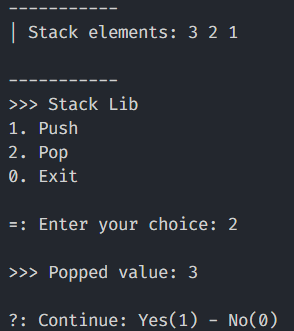
\includegraphics[width=\textwidth]{imgs/StackLinkedList/pop/normal.png}
		\caption{Normal test cases}\label{fig:stack_ll_pop_normal}
	\end{subfigure}
	\caption{Screenshots of Stack (Linked List version) `pop' operation.}\label{fig:stack_ll_pop_cases}
\end{figure}